% VUT FIT MITAI
% MSZ 2021/2022
% Author: Vladimir Dusek
% Login: xdusek27

%%%%%%%%%%%%%%%%%%%%%%%%%%%%%%%%%%%%%%%%%%%%%%%%%%%%%%%%%%%%%%%%%%%%%%%%%%%%%%%%

% Path to figures
\graphicspath{{tin/turingovy_stroje/figures}}

%%%%%%%%%%%%%%%%%%%%%%%%%%%%%%%%%%%%%%%%%%%%%%%%%%%%%%%%%%%%%%%%%%%%%%%%%%%%%%%%

\chapter{TIN~--~Turingovy stroje (jazyky přijímané TS, varianty TS, lineárně omezené automaty, vyčíslitelné funkce).}

%%%%%%%%%%%%%%%%%%%%%%%%%%%%%%%%%%%%%%%%%%%%%%%%%%%%%%%%%%%%%%%%%%%%%%%%%%%%%%%%

\section{Zdroje}

\begin{compactitem}
    \item \path{tin_2021_merged.pdf}
    \item \path{TIN_2020-10-20.mp4}
    \item \path{TIN_2020-10-27.mp4}
    \item \path{TIN_2020-11-03.mp4}
\end{compactitem}

%%%%%%%%%%%%%%%%%%%%%%%%%%%%%%%%%%%%%%%%%%%%%%%%%%%%%%%%%%%%%%%%%%%%%%%%%%%%%%%%

\section{Turingův stroj}

\begin{compactitem}
    \item Turingovy stroje jsou velmi robustní a jejich různé úpravy (determinismus, nedeterminismus, počet pásek, \dots) mají ekvivalentní vyjadřovací sílu z hlediska rozhodnutelnosti, ale z hlediska složitosti mají různou vyjadřovací sílu.

    \item Po pásce se můžeme pohybovat oběma směry. Páska je z prava nekonečná.

    \item Na TS lze nahlížet také jako na funkci, která má vstup počáteční pásku, pak nějaký výpočet (činnost TS) a jako výstup vrací stav pásky.
\end{compactitem}

\paragraph*{Definice TS} Turingův stroj (TS) je šestice $M = (Q, \Sigma, \Gamma, \delta, q_0, g_f)$, kde \begin{compactitem}
    \item $Q$ je konečná množina stavů;

    \item $\Sigma$ je vstupní abeceda (symboly, které se mohou vyskytovat na výchozím stavu pásky), \begin{compactitem}
        \item $\Delta \not\in \Sigma$;
    \end{compactitem}

    \item $\Gamma$ je pásková abeceda (symboly, které je možné zapisovat na pásku), \begin{compactitem}
        \item $\Sigma \subset \Gamma ~\land~ \Delta \in \Gamma ~\land~ L, R \not\in \Gamma$;
        \item Symbol $\Delta$ značí tzv. blank (prázdný symbol), který se vyskytuje na místech pásky,
        která nebyla ještě použita (může ale být na pásku zapsán i později).
    \end{compactitem}

    \item $\delta$ je přechodová funkce (parciální funkce), \begin{compactitem}
        \item $\delta : (Q - \{ q_f \}) \times \Gamma \rightarrow Q \times (\Gamma \cup \{ L, R \})$;
    \end{compactitem}

    \item $q_0$ je výchozí stav, \begin{compactitem}
        \item $q_0 \in Q$;
    \end{compactitem}

    \item $q_f$ je koncový stav, \begin{compactitem}
        \item $q_f \in Q$;
    \end{compactitem}
\end{compactitem}

\paragraph*{Konfigurace TS} Konfigurace TS je trojice $(q, \alpha, n) \in Q \times \{ \gamma \Delta^{\omega} ~|~ \gamma \in \Gamma \} \times \mathbb{N}$, kde \begin{compactitem}
    \item $q$ je aktuální stav;
    \item $\alpha$ značí stav pásky;
    \item $n$ značí pozici hlavy.
\end{compactitem}

\paragraph*{Počáteční konfigurace TS} Počáteční konfigurace je taková konfigurace $(q_0, \gamma \Delta^{\omega}, 0)$, kde $\gamma \Delta^{\omega}$ je výchozí stav pásky a $q_0$ je výchozí stav.

\paragraph*{Koncová konfigurace TS} Koncová konfigurace je taková konfigurace $(q_f, \gamma \Delta^{\omega}, n)$, kde $\gamma \Delta^{\omega}$ je stav pásky a $q_f$ je koncový stav.

\paragraph*{Přechod TS} Přechod TS $M$ (krok výpočtu) definujeme jako nejmenší binární relaci $\vdash$ takovou, že $\forall q_1, q_2 \in Q ~ \forall \gamma \in \Gamma^{\omega} ~ \forall n \in \mathbb{N} ~ \forall b \in \Gamma$: \begin{compactitem}
    \item $(q_1, \gamma, n) \vdash (q_2, \gamma, n + 1)$ pro $\delta(q_1, \gamma_n) = (q_2, R)$ -- operace posunu hlavy doprava při $\gamma_n$ po hlavou;

    \item $(q_1, \gamma, n) \vdash (q_2, \gamma, n - 1)$ pro $\delta(q_1, \gamma_n) = (q_2, L)$ -- operace posunu hlavy doleva při $\gamma_n$ po hlavou;

    \item $(q_1, \gamma, n) \vdash (q_2, s_b^n(\gamma), n + 1)$ pro $\delta(q_1, \gamma_n) = (q_2, b)$ -- operace zápisu symbolu $b$ při $\gamma_n$ po hlavou.
\end{compactitem}

Pro libovolný řetězec $\gamma \in \Gamma^{\omega}$ a číslo $n \in \mathbb{N}$ označme $\gamma_n$ n-tý symbol daného řetězce a označme $s_n^b(\gamma)$ řetězec, který vznikne z $\gamma$ záměnou $\gamma_n$ za $b$.

\paragraph*{Jazyk přijímaný TS} \begin{compactitem}
    \item Řetězec $w \in \Sigma^*$ je přijat TS $M = (Q, \Sigma, \Gamma, \delta, q_0, g_f)$, jesliže pro $M$ platí: $(q_0, \Delta \gamma \Delta^{\omega}, 0) \vdash^* (q_f, \gamma', n)$ pro nějaké $\gamma, \gamma' \in \Gamma^*$ a $n \in \mathbb{N}$.

    \item Množinu $L(M) = \{ w ~|~ w \text{ je přijat TS } M \} \subseteq \Sigma^*$ nazýváme jazyk přijímaný TS $M$.
\end{compactitem}

\begin{figure}[H]
    \centering
    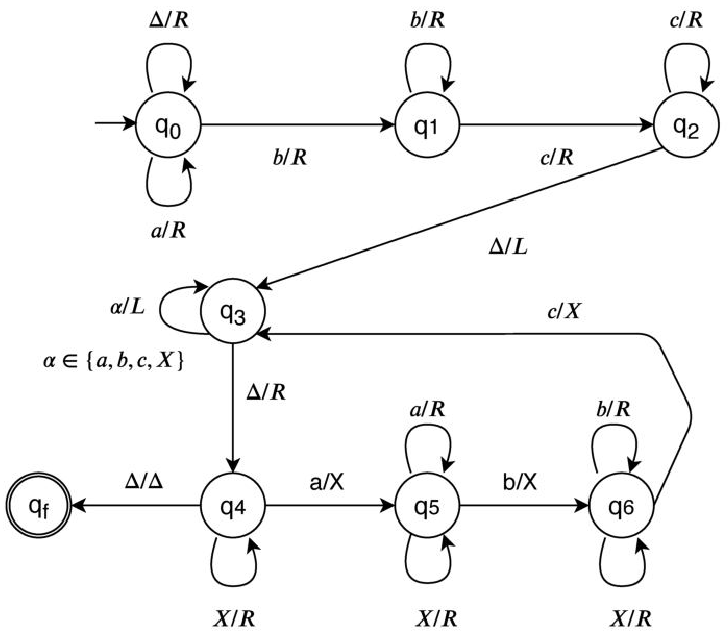
\includegraphics[width=0.8\linewidth]{ts_example.pdf}
    \caption{Příklad TS, který přijímá jazyk $L = \{ a^n b^n c^n ~|~ n > 0 \}$.}
\end{figure}

\paragraph*{Univerzální turingův stroj} Je možné sestrojit takový turingův stroj, který má vlastnost, že dokáže simulovat chování jiného Turingova stroje. Může fungovat jako interpret. Na vstupu přijme zakódovaný Turingův stroj (program) a vstup, který vykoná.

%%%%%%%%%%%%%%%%%%%%%%%%%%%%%%%%%%%%%%%%%%%%%%%%%%%%%%%%%%%%%%%%%%%%%%%%%%%%%%%%

\section{Varianty turingova stroje}

\subsection{Deterministický turingův stroj} Deterministický turingův stroj (DTS) je výchozí turingův stroj (DTS = TS).

\subsection{Vícepáskový turingův stroj}

Vícepáskový TS má stejnou (rozhodovací) vyjadřovací sílu jako jednopáskový TS (jsou mezi sebou převoditelné). Formálně to znamená, že pro každý $k$-páskový TS $M$ existuje jednopáskový TS $M'$ takový, že $L(M) = L(M')$. Myšlenka důkazu spočívá v tom, že $k$ pásek můžeme simulovat jednou. Jeden symbol na pásce potom bude mít formu $2k$-tice. Pro každou pásku jsou potřeba 2 prvky v n-tici, protože v jedné je třeba si udržovat pozici hlavy. Myšlenka je na obrázku.

\begin{figure}[H]
    \centering
    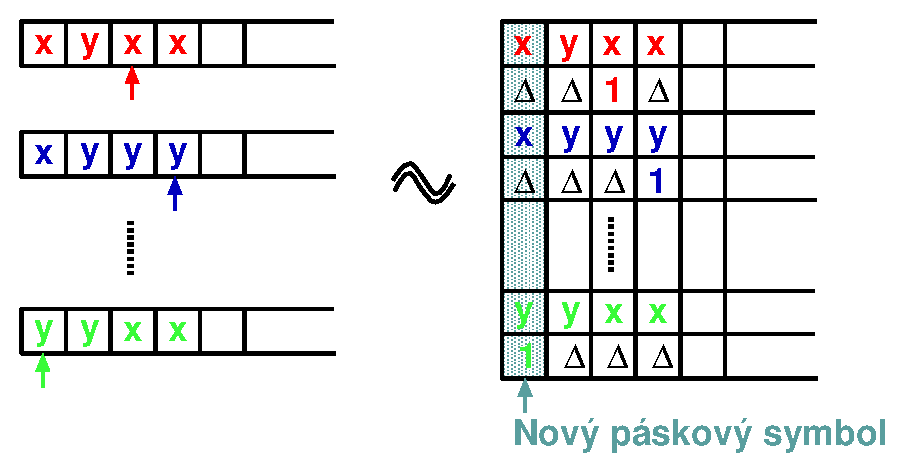
\includegraphics[width=1\linewidth]{ts_vicepaskovy_dukaz.pdf}
    \caption{Myšlenka převodu vícepáskového TS na jednopáskový.}
\end{figure}

\paragraph*{Definice} \todo{todo}

\paragraph*{Příklad} Příklad vícepáskového TS.

\begin{figure}[H]
    \centering
    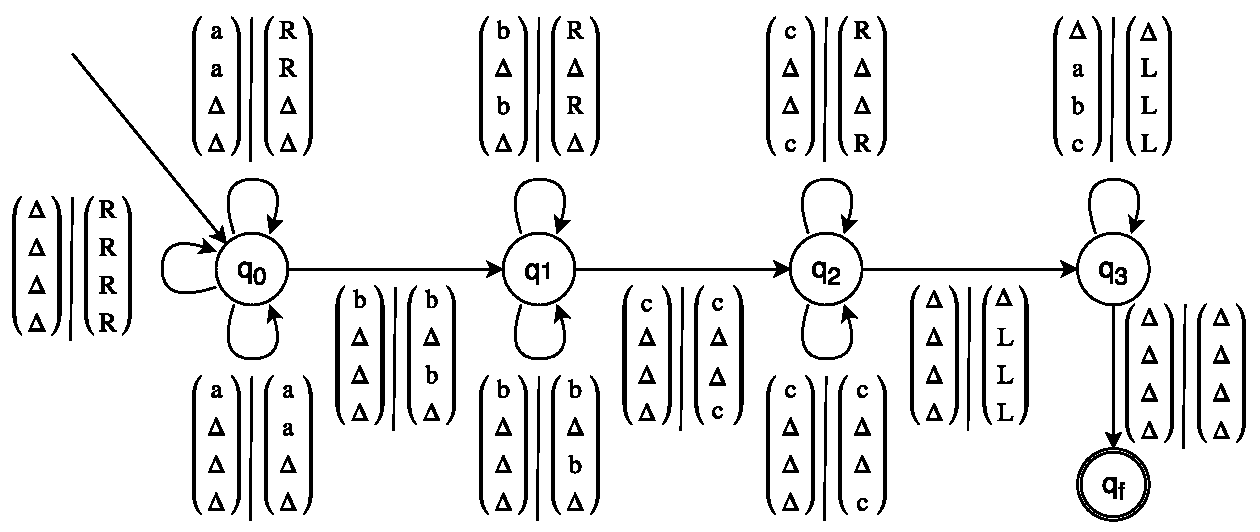
\includegraphics[width=1\linewidth]{ts_vicepaskovy_example.pdf}
    \caption{Příklad 4-páskový TS, který přijímá jazyk $L = \{ a^n b^n c^n ~|~ n > 0 \}$.}
\end{figure}

\subsection{Nedeterministický turingův stroj}

Nedeterministický TS (NTS) má stejnou (rozhodovací) vyjadřovací sílu jako DTS (jsou mezi sebou převoditelné). Formálně to znamená, že pro každý NTS $M$ existuje DTS $M'$ takový, že $L(M) = L(M')$. Myšlenka důkazu spočívá v tom, že strom běhů NTS prohledáváme do šířky (jelikož běh může obsahovat smyčky). Konkrétně, NTS $M$ budeme simulovat třípáskovým DTS. Význam jednotlivých pásek tohoto
stroje je následující: \begin{compactitem}
    \item Páska 1 obsahuje vstupní řetězec.
    \item Páska 2 je pracovní páska. Obsahuje kopii pásky 1 ohraničenou vhodnými speciálními značkami. Po neúspěšném pokusu o přijetí je její obsah smazán a obnoven z první pásky.
    \item Páska 3 obsahuje kódovanou volbu posloupností přechodů; při neúspěchu bude její obsah nahrazen jinou posloupností.
\end{compactitem}

\paragraph*{Definice} \todo{todo}

\paragraph*{Příklad} Příklad nedeterministického TS, kde nedeterminismus může přinést značné zjednodušení, je TS, který přijímá jazyk $L = \{ ww ~|~ w \in \Sigma^* \}$.

\subsection{Úplný turingův stroj}

Úplný turingův stroj je takový TS, který pro libovolný vstup zastaví, a buď přijme nebo odmítne (nemůže se zacyklit). Úplné turingovy stroje mají menší (rozhodovací) vyjadřovací sílu než obecný turingův stroj.

\paragraph*{Rekurzivně vyčíslitelné jazyky} Jazyky přijímané turingovými stroji se nazývájí rekurzivně vyčíslitelné ($\mathcal{L}_1, REL, \mathcal{L}_{RE}$).

\paragraph*{Rekurzivní jazyky} Jazyky přijímané úplnými turingovými se nazývají rekurzivní ($RL, \mathcal{L}_{Rec}$). Platí $2^{\Sigma^*} \subset \mathcal{L}_{RE} \subset \mathcal{L}_{Rec} \subset \mathcal{L}_1$.

%%%%%%%%%%%%%%%%%%%%%%%%%%%%%%%%%%%%%%%%%%%%%%%%%%%%%%%%%%%%%%%%%%%%%%%%%%%%%%%%

\section{Lineárně omezený automat}

\todo{todo}

%%%%%%%%%%%%%%%%%%%%%%%%%%%%%%%%%%%%%%%%%%%%%%%%%%%%%%%%%%%%%%%%%%%%%%%%%%%%%%%%

\section{Vyčíslitelné funkce}

\todo{todo}
